\chapter{Biologia Molecular e Bioinformática}
 
\indent Neste capítulo serão descritos os conceitos básicos da biologia molecular. A seção \ref{aceidosNucleicos} define tais estruras e diferencia DNA de RNA por suas configurações e funções. A seção \ref{sinteseDeProteina} define as proteínas, apresenta seus quatro tipos diferentes e descreve o processo de sintetização de proteína. Por fim, a seção \ref{bioinformatica} estabelece os conceitos básicos dessa área, além de apontar os problemas atuais enfrentados nela.





%% ================================================================================================================== %%


\section{Ácidos Nucléicos} \label{aceidosNucleicos}

\indent Os ácidos nucléicos são biomoléculas responsáveis pelo armazenamento, transmissão e tradução das informações genéticas dos seres vivos. Isto é possível devido ao processo de síntede de proteínas que permite, assim, a base da herança biológica.Os acidos nucléicos são polímero, macromoléculas formadas por estruturas menores chamadas monômeros, que nesse caso são nucleotídeos. Nucleotídeos são compostos de três elementos: um radical fosfato (HPO$_{4}$), uma pentose, ou seja, um monossacarídeo formado por cinco átomos de carbono, e uma base nitrogenada. Existem cinco tipos de bases nitrogenadas que podem compor um nucleotídeo: Adenina(A), Timina(T), Citosina(C), Guanina(G) e Uracila(U). \\

\begin{figure}[h]
    \centering
    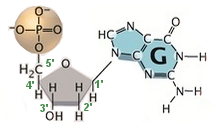
\includegraphics[width=0.5\textwidth]{nucleotideo.png}
    \caption{imagem de um nucleotídeo e das bases nitrogenadas. Mostrar backbone da pentose 1'...5'. Adaptado de : \cite{dnadiscovery08}. }
    \label{fig:Nucleotideo}
\end{figure} 

\indent Na figura \ref{fig:Nucleotideo}, observa-se que no \textit{backbone} do nucleotídeo existe uma numeração de 1' à 5', que representam os carbonos presentes na pentose. Para a criação de uma fita de ácido nucléico, no processo de polimerização fomar-se uma ligação fosfodiéster entre o carbono da posição 5' do \textit{backbone} de um nucleotídeos e o carbono de posição 3' do \textit{backbone} de outro \cite{setubal97}. Por definição o sentido da leitura de uma fita de ácido nucléido é 5' $\rightarrow$ 3', o que é deve ser levado em consideração ao se fazer interpretação de dados do material genético.

\indent Dois tipos de ácidos nucléicos são encontrados nos seres vivos: ácido desoxirribonucleico (DNA) e ácido ribonucleico (RNA). Eles diferenciam-se tanto na estrutura do \textit{backbone} e nas bases nitrogenadas, quanto em suas funções. A seguir serão apresentadas as definições de DNA e RNA.

\subsection{DNA} \label{aceidosNucleicos:dna}

\indent Os DNAs (ou ADN - Ácido Desoxirribonucleico) são as biomoléculas que armazenam as informações referentes ao funcionamento de todas as células dos seres vivos de maneira específica: sequências de pares de bases nitrogenadas. Nesse sentido, além de haver a ligação fosfodiéster entre os nucleotídeos, cada um também se liga a partir de suas bases nitrogenadas, formando assim um eixo helicoidal tridimensional chamada de dupla hélice \cite{setubal97}. Esta estrutura foi descoberta em 1953, pelo biólogo James Watson e pelo físico Francis Crick \cite{dnadiscovery08}, porém os ácidos nucléicos já eram estudado desde 1869 na Suíça pelo químico-fisiológico Friedrich Miescher.

\indent Em relação à estrutura dos monômeros do DNA, o \textit{backbone} dos nucleotídeos é uma desoxirribose, indicada na figura \ref{fig:EstruturasDoDNA}. Para a formação da dupla hélice, os pares são feitos com uma base nitrogenada do grupo de purinas, composto orgânico que possui um anel duplo de carbono, e outra base do grupo de pirimidinas, composto orgânico que possui um anel simples de carbono. No caso do DNA, somente quatro das cinco bases são empregadas: as purinas Adenina(A) e Guanina(G), que se ligam com as pirimidinas Timina(T) e Citosina(C) respectivamente. Desta forma, A e T são bases complementares, assim como G e C. Uma fita de DNA pode conter centenas de milhões de nucleotídeos.

\indent A representação do DNA, seja nos livros ou computacionalmente, é dada por um par em paralelo de strings de letras A, T, G e C. Como explicado no início dessa seção, o sentido padrão da leitura de uma fita é de 5' $\rightarrow$ 3', mas no caso do DNA, as hélices são dispostas de maneira antiparalela, ou seja, uma é lida de 5' $\rightarrow$ 3' e a outra, de 3' $\rightarrow$ 5'. Observa-se que a partir de uma hélice, pode-se inferir a sequência de sua hélice complementar. Seja, por exemplo, uma hélice H1 igual a AGTAAGC; então H2 em seu sentido oposto é H2' igual a TCATTCG, e no sentido regular, igual a GCTTACT. A figura \ref{fig:EstruturasDoDNA} apresenta a estrutura do DNA como explicada nesta seção. \\

\begin{figure}[h]
    \centering
    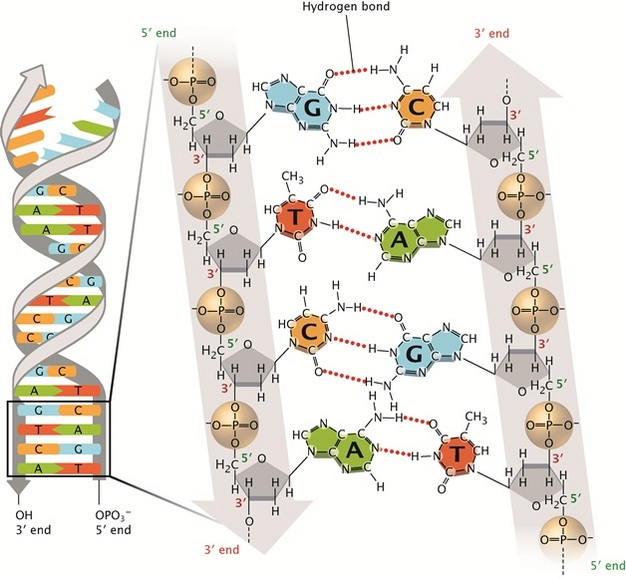
\includegraphics[width=0.7\textwidth]{dnaEstrutura.jpg}
    \caption{Adaptado de : \cite{dnadiscovery08} }
    \label{fig:EstruturasDoDNA}
\end{figure} 


\subsection{RNA} \label{aceidosNucleicos:rna}

\indent Os RNAs são biomoléculas semelhantes ao DNA, porém contam com três diferenças básicas. A primeira é a estrutura do \textit{backbone} dos nucleotídeos, que é composta por uma ribose ao invés de um desoxirribose. A segunda difereça é em relação às bases nitrogenadas, onde a pirimidina Uracila(U) substitui a Timita(T). Por fim, o RNA é formado por apenas uma hélice tridimensional.

\indent Existem três tipos de RNAs presentes no citoplasma - espaço entre a membrama plasmática e o núcleo da célula. 
Cada um possui funções específicas que serão detalhadas na seção \ref{sinteseDeProteina:transcricaoTraducaoSintese}. Em suma, O RNA mensageiro (mRNA) é responsável pela transferência de informação do DNA para o RNA ribossômico (rRNA), que por sua vez irá desanexar a proteína do RNA transportador (tRNA) combinando-o com o rRNA, executando assim, a síntese de proteína.



%% ================================================================================================================== %%

\section{Síntese de Proteína} \label{sinteseDeProteina}



\subsection{Proteína} \label{sinteseDeProteina:proteina}

\indent As proteínas são biomoléculas com diversas responsabilidades no corpo dos seres vivos. 
Se fizerem parte do no grupo de proteínas fibrosas, como o colágeno, irão compor a estrutura do corpo e para isso precisam ser resistentes e insolúveis em água. Caso estejam no grupo de proteínas globulares, como a hemoglobina, realizarão processos dinâmico pelo corpo tais como transportações e cataliações \cite{profangela11}.  Cada tarefa é realizada por um proteína com uma estrutura específica e otimizada pra tal.

\indent Assim como os ácidos nucléicos, as proteínas são polímeros, macromoléculas cujos monômeros são aminoácidos. Aminoácidos são moléculas que possuem cinco componentes: amina (NH$_{2}$), carbono (C), hidrogênio (H), ácido carboxílico (COOH) e uma cadeia lateral que funciona como identificador de cada um dos 20 tipos de aminoácidos presentes nos seres vivos. A maneira como eles são criados será explicada com mais detalhes na subseção \ref{sinteseDeProteina:transcricaoTraducaoSintese}, pois envolve um processo complexo de síntese de proteína executado pelo ribossomo. A ligação, ou polimerização, de dois aminoácidos é feita unindo a amida de um com o ácido carboxílico do outro, liberando uma molécula de água (H$_{2}$O) e formando uma cadeia chamada de dipeptídeo. Como houve liberação de água na ligação, o dipeptídeo não é formado por aminoácidos, mas sim resíduos dos mesmos. Nesse sentido, cadeias peptídicas de 100 à 5000 diferentes resíduos aminoácidos, ou cadeia polipeptídicas,  constituem a proteína.

\indent Existem quatro estruturas para caracterização de uma proteína \cite{setubal97}. A mais simples é chamada de estrutura primária e é composta por uma sequência linear de resíduos aminoácidos. A estrutura secundária é tridimensional e estabiliza-se por meio de ligações de hidrogênio na cadeia principal, chamada de \textit{backbone}. Dependendo da disposição dos resíduos de aminoácidos, esta cadeia pode se dar forma de hélice ou em forma de folha. A estrutura terciária é dada pela união de várias estruturas secundárias e, por fim, a estrutura quaternária é composta de múltiplas estruturas terciárias \cite{drug09}. A figura \ref{fig:EstruturasDaProteina} ilustra os quatro tipos de proteínas descritos.

\begin{figure}[h]
    \centering
    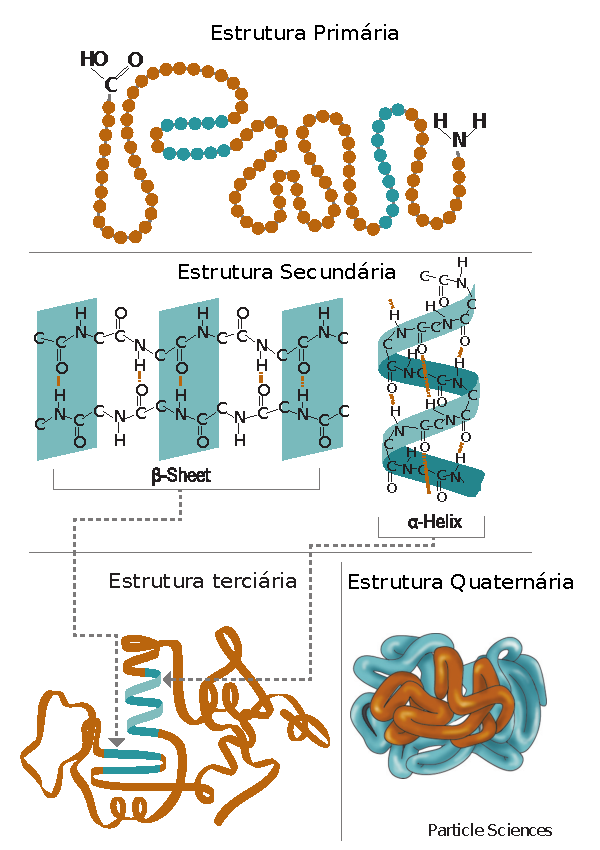
\includegraphics[width=0.6\textwidth]{EstruturasDaProteina.pdf}
    \caption{Adaptado de : \cite{drug09} }
    \label{fig:EstruturasDaProteina}
\end{figure}

\subsection{Código Genético} \label{sinteseDeProteina:codigoGenetico} 

\indent No núcleo de cada célula eucariota, ou no citoplasma das células procariotas, estão localizados as moléculas de DNA, chamadas individualmente por \textbf{cromossomo}. O número de cromossomos em cada célula varia por espécie. No caso dos chimpanzés, o núcleo das células possui 48 cromossomos e no caso dos seres humanos, 46. Note que não existe relação entre o grau evolutivo das espécies e o número de cromossomos nas células.

\indent Um cromossomo pode ser representado por vários trechos contíguos de DNA, sendo que cada trecho é chamado de \textbf{gene}, ou locus - local fixo no cromossomo. Portanto, pode-se afirmar que o cromossomo é um conjunto (ou lista) de genes. No caso dos seres humanos, o número de genes em cada célula gira em torno de 22 mil \cite{pertea2010}, e o genoma humano possui em média 3 bilhões de pares de bases. Poderíamo inferir, então, que a média de pares de bases por gene é de $\frac{3.000.000.000}{22.000} \simeq 136.000$, porém este cálculo é muito generalizado e equivocado, uma vez que os genes possuem tamanhos diferentes, onde o maior possui 250 milhões de pares, enquanto o menor possui apenas 50 milhões, no caso dos seres humanos \cite{nussbaum08}. Um gene, por sua vez, pode ser representado por vários trechos de três pares de base, sendo que cada trecho é chamado de \textbf{códon}.

\indent Normalmente cada proteína é formada a partir de um gene particular. Mais especificamente, cada aminoácido da proteína é formado a partir de um códon do gene. Entretanto, existem 64 códon possíveis ($4_{ParesDeBase} ^3$) mas somente 20 aminoácidos a serem codificados. Nesse sentido, é comum haver mais de um códon correspondendo à um aminoácio. Além disso, 3 destes códons são responsáveis por indicar o final de uma proteína. O mRNA é encarregado de transportar a informação da sequência correta para construção de proteína, em forma de sequência de códons. A tabela \ref{tabelaCodigoGenetico} que apresenta a correspondência entre códons e aminoácios é chamada de código genético \cite{setubal97}, e a tabela \ref{tabelaAminoacidos} apresenta o código genético codificado em letras do alfabeto utilizado atualmente para comparação entre proteínas. Note que as bases nitrogenadas são do RNA, e não do DNA, pois é a molécula do primeiro que faz a conexão entre DNA e a proteína, num processo que será explicado na subseção \ref{sinteseDeProteina:transcricaoTraducaoSintese}.

\indent A partir destas tabelas, podemos montar o seguinte exemplo: Suponha que a palvra GENETICA seja uma proteína. Então existe uma configuração de aminoácidos que forma essa proteína, e ela pode ter a forma: \\ 
\indent GENETICA $\leftarrow$ Glicina - Glutamano - Metionina - Glutamano \\
\hspace*{3.4cm}  Treonina - Isoleucina - Cisteina - Alanina \\
\indent GENETICA $\leftarrow$ Gly - Glu - Asn - Glu - Thr - Ile - Cys - Ala \\
\indent GENETICA $\leftarrow$ GGG - GAG - AAC - GAA - ACG - AUC - UGC - UCC \\


\begin{table}[h!] 
\centering
%\captionsetup{labelsep=space,justification=justified,singlelinecheck=off}
\caption{Código Genético} \label{tabelaCodigoGenetico}
\begin{tabular}{|c|c|c|c|c|c|c|c|}
\hline
 \multirow{2}{*}{ \begin{tabular}[x]{@{}c@{}} Primeira \\ Posição \end{tabular} } & 
 \multicolumn{4}{|c|}{Segunda Posição} & 
 \multirow{2}{*}{ \begin{tabular}[x]{@{}c@{}} Terceira \\ Posição \end{tabular} }\\  \cline{2-5}
 & G & A & C & U &  \\ \hline
 
 \multirow{5}{*}{G} & Gly & Glu & Ala & Val & G \\ 
 					& Gly & Glu & Ala & Val & A \\ 
% 					& & & & & 					 \\ 
 					& Gly & Asp & Ala & Val & C \\ 
 					& Gly & Asp & Ala & Val & U \\ \hline 
 					
 \multirow{5}{*}{A} & Arg & Lys & Thr & Met & G \\ 
 					& Arg & Lys & Thr & Ile & A \\ 
% 					& & & & & 					 \\ 
 					& Ser & Asn & Thr & Ile & C \\ 
 					& Ser & Asn & Thr & Ile & U \\ \hline 
 					
 \multirow{5}{*}{C} & Arg & Gln & Pro & Leu & G \\ 
 					& Arg & Gln & Pro & Leu & A \\ 
% 					& & & & & 					 \\ 
 					& Arg & His & Pro & Leu & C \\ 
 					& Arg & His & Pro & Leu & U \\ \hline 
 					
 \multirow{5}{*}{U} & Trp & \textbf{FIM} & Ser & Leu & G \\ 
 					& \textbf{FIM} & \textbf{FIM} & Ser & Leu & A \\ 
% 					& & & & & 					 \\ 
 					& Cys & Tyr & Ala & Phe & C \\ 
 					& Cys & Tyr & Ala & Phe & U \\ \hline 
 
\end{tabular}
\end{table}


\begin{table}[h!] 
\centering
%\captionsetup{labelsep=space,justification=justified,singlelinecheck=off}
\caption{Aminoácidos codificados} \label{tabelaAminoacidos}
\begin{tabular}{|c|c|c|c|} \hline
& Aminoácido & Abreviação & Código no alfabeto  \\  \hline
1 & Alanina & Ala & A \\ 
2 & Cisteina & Cys & C \\ 
3 & Aspartano ou Ácido aspártico & Asp & D \\ 
4 & Glutamato ou Ácido glutâmico & Glu & E \\ 
5 & Fenilalanina & Phe & F \\ 
6 & Glicina ou Glicocola & Gly & G \\ 
7 & Histidina & His & H \\ 
8 & Isoleucina & Ile & I \\ 
9 & Lisina & Lys & K \\ 
10 & Leucina & Leu & L \\ 
11 & Metionina & Met & M \\ 
12 & Asparagina & Asn & N \\ 
13 & Prolina & Pro & P \\ 
14 & Glutamina & Gln & Q \\ 
15 & Arginina & Arg & R \\ 
16 & Serina & Ser & S \\ 
17 & Treonina & Thr & T \\ 
18 & Valina & Val & V \\ 
19 & Tripofano & Trp & W \\ 
20 & Tirosina & Tyr & Y \\ \hline
 
\end{tabular}
\end{table}


% Mudar para "Dogma central" e falar das 5 fases, com ênfase em transcrição e tradução
\subsection{Transcrição e tradução} \label{sinteseDeProteina:transcricaoTraducaoSintese}

% PROCARIÓTAS
\indent Para finalizar esta seção, serão descritos os processos de transcrição, tradução e síntese de proteína. O início de cada gene é reconhecido ou em uma região chamada de \textit{promotor} ou, alternativamente, pelo códon AUG. A partir de então, uma cópia deste gene, ou \textit{clusters} de genes, é feita sobre uma molécula de mRNA que, por consequência, obterá a mesma sequência que uma das cadeias do gene, porém trocando os U's por Ts, através deste processo chamado de \textbf{transcrição}. A cadeia que se assemelha ao produto mRNA é chamado de cadeia codificadora (lida de 5' para 3'), enquanto a cadeia oposta é chamada de cadeia de molde (lida de 3' para 5'). Para denotar a orientação de cada cadeia codificadora, os termos \textit{upstream} e \textit{downstream} são utilizados. Observe que o promotor é o \textit{upstream} do gene, pois reconhece seu início.

% EUCARIOTAS

\indent No caso dos organismos eucariotas, em que o núcleo da célula está elvolto na membrana nuclear, os fragmentos do gene que não serão utilizados para síntese de proteína, íntrons, são descartados do mRNA após a transcrição e aqueles que serão usados, éxons, são mantidos. Observe que a partir do momento em que o gene foi dividido entre íntrons e éxons, ele muda sua denominação e passa a se chamar DNA genômico. Nesse sentido, a sequência de somente éxons também recebe outro nome: DNA complementar, ou cDNA.

\indent Após esta separação, o mRNA deixa o núcleo celular e inicia a \textbf{transcrição reversa} no citoplasma. O processo ocorre no interior de uma organela celular chamada de ribossomo, constituído de proteínas e rRNA e cuja função é construir a molécula de proteína a partir de duas entradas, o mRNA e tRNA. A estrutura do tRNA é tal que de um lado se encaixa exatamente um códon e no oposto, seu aminoácido correspondente. O processo de \textbf{tradução} se dá da seguinte maneira: a medida em que o mRNA passa pelo interior do ribossomo, este atrai quaisquer tRNAs das proximidades cujos códons sejam correspondentes ao da subsequência corrente do mRNA. No momento em que o códon do tRNA se conecta com um dos códons do mRNA, o aminoácido que estava fixado naquele é liberado e agregado, com o auxílio da catálise de uma enzima, na molécula de proteína em desenvolvimento. Esta é finalmente completa quando o mRNA aprensenta um códon de parada, pois nenhum tRNA possui correspondência para tal \cite{setubal97}.


\section{Bioinformática} \label{bioinformatica}

\indent O que é, quando surgiu

\indent Quero amplificar um fragmento pra estudar : PCR

\indent Quero comparar dois transcriptomas : Microarry

\indent Quero sequenciar : Sanger (antigo) e Illumina (novo)

\indent \cite{mardis08}, Annotations (interseções)


\subsection{Desafio das ômicas}

\indent Nas últimas duas décadas, o progresso tecnológico no sequenciamento genômico ultrapassou o crescimento previsto pela Lei de Moore \cite{berger13}, a qual afirma que as capacidades de processamento e armazenamento de um computador dobram a cada 18 meses. Nesse sentido, algumas áreas de sufixo "ômica", como, por exemplo, genômica, transcriptômica, interatômica, enfrentam desafios computacionais atualmente.

\indent Em relação ao procesamento, armazenamento e recuperação  de dados, existem três problemas principais sendo enfrentados. O primeiro se refere a construção do genoma, que requer a associação se milhões de pequenas sequências e memória na ordem de terabytes; O segundo desafio é o alinhamento de sequências, que também é um processo oneroso se utilizado a técnica de combinação de cadeias, letra por letra; existem técnicas de compressão de dados que encurtam as sequências e outros de programação paralela que aceleram este processo. O terceiro desafio é a (des)compressão de dados para armazenamento e processamento, visto que a análise computacional do material requer as sequências genômicas originais.

\indent Em relação aos desafios da área transcriptômica, referente aos RNA's, os problemas são a identificação de expressões, ou características fenótipas, de células específicas, especialmente tecidos, pois são difíceis de de interpretar; identificação de genes e módulos regulatórios, um grupo de gene com funções biológicas específicas; identificação das alterações nas expressões genéticas em doenças \cite{berger13}.

\indent Já em relação à área de interatoma, referente à interações entre proteínas que ocorrem nas células do organismo \cite{bonetta2010}, os desafios são analisar os conjuntos de dados genômicos heterogêneos e elaborar análise interatoma de conjunto de dados de doenças. Geralmente as redes interatômicas são representadas por grafos, onde os nós são componentes biológicos e as arestas são as interações entre eles.

\subsection{Visualização de dados ômicos}